\chapter{Planning and Methodology}
\label{cap:plan}

\section{Feasibility Study}

Before initiating any project, it is of utmost importance to conduct a comprehensive analysis of relevant factors to gauge the likelihood of accomplishing successful outcomes. While estimating the complexity associated with developing, deploying, and maintaining machine learning (ML) systems is indeed a challenging task, it is essential to recognize that this project encompasses not only the research aspect but also significant software and infrastructure development. \\

This project requires a careful balancing act, as it involves dedicating efforts to both the research and practical implementation aspects. The development of robust software and infrastructure is crucial to support the successful integration of the deep learning models and ensure their efficient deployment and maintenance. This integration can be intricate and demanding, as it requires a deep understanding of both the ML algorithms and the software engineering principles. \\

In light of these additional dimensions, the study not only aims to evaluate the feasibility of utilizing deep learning techniques but also strives to address the complexities inherent in developing a well-rounded solution. Furthermore, the evaluation will consider the available data and resources to assess the potential of achieving satisfactory results. 

\section{Technical Study}

The journey begins with research, a dynamic element that evolves and gains strength through continuous investigation. While it is impossible to guarantee the achievement of all objectives, the way wee see it, there are three fundamental pillars that must be addressed in advance. \\

\vspace{0.5cm}
\textbf{Defining the Use Case} \\

\textit{A perfect use case outlines a project that is precisely defined, quantifiable, attainable, and possesses clearly identified users and value.} \\

Academic researchers may find satisfaction in uncovering effective solutions that contribute to publications and secure additional funding. Yet, this thesis aims to ensure the successful implementation of a CAD (Computer-Aided Diagnosis) infrastructure specifically designed for classifying melanoma, with the intention of deploying it in real-world scenarios I need to look further than just the pure research. \\

It is important to note that the scope of this project does not encompass the commercialization of a product or service. Yet the intention of creating services from the primary focus study is present. As a consequence of the use case the technical study is based on analyzing which
technology and equipment are necessary for carrying out experiments in
the most efficient way. \\

\vspace{0.5cm}
\textbf{Equipment and Technical Knowledge} \\

Equipment and technical knowledge are interdependent and collectively contribute to the success of a machine learning project. \\

In a deep learning project, both the availability of suitable equipment and technical knowledge are essential. The correct equipment, including high performance computing resources and data collection devices, facilitates efficient data handling, prepossessing, model training, and deployment. Simultaneously, technical knowledge plays a vital role in effectively leveraging the available equipment. Understanding diverse machine learning algorithms and methodologies assists in selecting the most appropriate approaches for the problem at hand. Additionally, it is crucial to acknowledge the knowledge required to create other services that accompany the project. \\

\vspace{0.5cm}
\textbf{Importance of the Dataset} \\

The success of a project like this one depends not only on the quantity but also on the quality of the data. Data is essential for any deep learning model to learn effectively. Therefore, it is vital to invest time in acquiring an optimal image data-set that possesses sufficient data volume, annotation, truth, and reusability. \\

For computer-based image recognition and analysis, high-quality data is necessary. The objective is to gather data from various patient populations to ensure that the data-set is diverse and accurately represents different disease states and outcomes. Often, healthcare organizations engage medical experts to review and label the data to prevent inaccurate labels and ensure the data-set's significance, as is the case in this project.

\section{Economical Study}

\vspace{0.5cm}
\textbf{Equipment Cost} \\

Equipment cost pertains to the expenditure incurred on hardware and software licenses necessary for the project. \\

The hardware and software used in the project are listed in the \textit{Table \ref{table:equipment_cost}}.

\begin{table}[H]
\centering
\begin{tabular}{| l | c | c | c |}
\hline
\multicolumn{1}{|c|}{Component} & \multicolumn{1}{c|}{Units} & \multicolumn{1}{c|}{Unit Price} & \multicolumn{1}{c|}{Cost} \\
\hline
Computer & 1 & \$800 & \$800 \\
\hline
Software (Pytorch, Svelte, FastAPI, etc) & 1 & \$0 & \$0 \\
\hline
Tesla T4, 16GB (GPU)* & 1 & \$2000 & \$2000 \\
\hline
Nvidia A100, 80GB (GPU)* & 1 & \$15000 & \$15000 \\
\hline
\end{tabular}
\caption[The Cost of Components.]{\textit{The Cost of Components. Components marked with (*) were not paid for out of my own pocket; instead, they were borrowed from VICOROB or Google Services.}}
{\label{table:equipment_cost}}
\end{table}

\vspace{0.5cm}
\textbf{Human Resources} \\

In this section, a hypothetical scenario is presented, illustrating multiple work profiles contributing to the project and the associated costs for each service. However, it is important to note that in reality, all tasks were performed by a single individual. \\

Below, the roles required to achieve the thesis are presented along with their explanations. \\

\begin{itemize}
    \item \textbf{Data Scientist} \\
    
Data scientists focus on managing and analyzing data throughout the project. They acquire relevant datasets, preprocess the data, develop deep learning models, train and evaluate models, and deploy them in production environments (some cases). \\

The average hourly wage for a Data Scientist in United States is \textbf{\$36} \cite{SalaryDataScientist}. \\

\item \textbf{Research Scientist} \\
    
Research scientists focus on the exploration and innovation aspects of deep learning projects. Their roles typically include, literature review: Research scientists survey existing literature, stay updated with the latest advancements in deep learning, and identify relevant research papers or techniques that can be applied to the project. Innovation and Experimentation: They contribute to the development of novel deep learning architectures, techniques, or algorithms to address specific project challenges or improve model performance. \\

The average hourly wage for a Computer Research Scientist in United States is \textbf{\$121.163} \cite{SalaryResearchScientist}. \\

\item \textbf{Data Engineer} \\
    
Data engineers are typically in charge of creating the user interface (UI) components of the application that interact with the deep learning models. But the most important tasks handled by this profile would be data pre-processing, API development, and model integration. They would build the necessary APIs to communicate with the deep learning models. \\

The average hourly wage for a Data Engineer in United States is \textbf{\$48} \cite{SalaryDataEnginner}. \\

\end{itemize}

\newpage

\begin{table}[H]
\centering
\begin{tabular}{| l | c | c | c | c |}
\hline
\multicolumn{1}{|c|}{\textbf{Task}} & \multicolumn{1}{c|}{\textbf{Profile}} & \multicolumn{1}{c|}{\textbf{Time}} & \multicolumn{1}{c|}{\textbf{Cost}} \\
\hline
Definition and boundaries of the project & Research Scientist & 50h & \$6,081.5\\
\hline
Data collecting & Data Engineer & 10h & \$480\\
\hline
Data preprocessing & Data Engineer & 10h & \$480 \\
\hline
Data analysis and visualization & Data Scientist & 30h & \$1,080\\
\hline
Model development & Research Scientist & 60h & \$7,297.8 \\
\hline
Model training & Data Scientist & 80h & \$2,880 \\
\hline
Model optimization & Data Scientist & 120h & \$4,320 \\
\hline
Models reports & Data Scientist & 20h & \$720 \\
\hline
CAD infrastructure & Data Engineer & 220h & \$10,560 \\
\hline
Infrastructure deployment & Data Engineer & 20h & \$960 \\
\hline
Documentation & Research Scientist & 100h & \$12,163 \\
\hline
\textbf{Total} &    &  \textbf{720h} & \$47,022.3 \\
\hline
\end{tabular}
\caption[Human Resources Estimated Cost.]{\textit{Human Resources Estimated Cost.}}
{\label{table:human_resources_cost}}
\end{table}

The tasks, along with the assigned profile and estimated cost, are presented in \textit{Table \ref{table:human_resources_cost}}. \\

\vspace{0.5cm}
\textbf{Methodology} \\

The project methodology employed in this endeavor follows a continuous process that builds upon previous approaches. Additionally, the project incorporates the concept of utilizing idle time effectively. For instance, during the training of models, there are periods of idle time, which I exploit by concurrently working on tasks related to developing the entire infrastructure. This approach allows for maximizing productivity throughout the project. The various stages involved in the methodology are as follows: \\

\begin{enumerate}

    \item Identifying the problem and establishing the research objectives.
    \item Conducting background research by reviewing prior publications addressing similar or related issues.
    \item Choosing a programming language and framework.
    \item Study of the characteristics and distribution of the working data-set.
    \item Familiarizing oneself with the tools and frameworks will be utilized.The term "equipment cost" pertains to the expenditure incurred on hardware and software licenses necessary for this project.
    \item Breaking down the project into smaller tasks.
    \item Selecting a specific task.
    \item Trying to implement the task in a smart manner.
    \item Developing the task.
    \item Make GPU do its job for certain number of epochs (Iddle).

        \begin{itemize}
            \item Choosing or resuming a develop task (API, UI or Virtualization).
            \item Developing process.
                \begin{itemize}
                    \item Developing interruption because model is already trained or because early stopped. Go to point 11. 
                     \item If there are remaining tasks, choose a new develop task.
                \end{itemize}
        \end{itemize}

    
    \item Evaluating whether the results meet the expectations.

        \begin{itemize}
            \item If the results fall short of expectations, return to step 8.
            \item If the results meet the expectations, proceed to step 12.
        \end{itemize}

    \item Collecting the necessary artifacts and presenting the results in a clear and appealing manner.

    \item Deploy models.

    \item Deploy the CAD system infrastructure.

    \item Write down the report.
    
\end{enumerate}

\textit{Figure \ref{fig:flux_development}} Illustrates the previous process by making use of a diagram. 

\newpage


\begin{figure}[H]
\centering
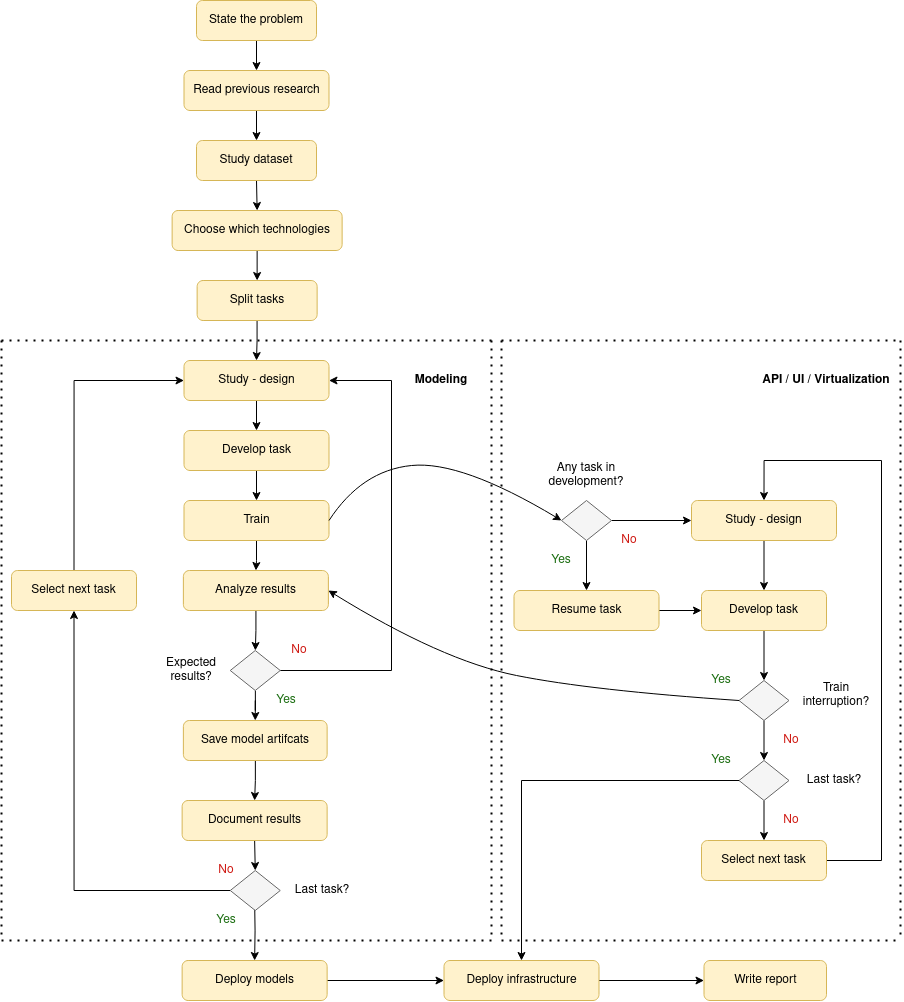
\includegraphics[width=\textwidth]{imatges/planing_and_methodology/EmplyedMethodology.png}
\caption[Activity Diagram Describing the Methodology.]{\textit{Activity Diagram Describing the Workflow Methodology: Notice that the right workflow is executed every time models are trained and returns to the model evaluation once the models have been trained to analyze results. Illustration by Author}}
{\label{fig:flux_development}}
\end{figure}


\newpage


\section{Planning}

This thesis was developed under an inter-ship in the Accenture SL company, under the category of Research, innovation, and development. The intern-ship was thought to conduct the Master thesis at the University of Girona. We also had the help from VICOROB laboratory which is the Computer Vision and Robotics Research Group of the University of Girona. This thesis runs under the guidance of Dr. Rafel Garcia (UdG) and Luis Llopis (Accenture SL) from 1st of December, 2022 to 12th of July of 2023. \\

From now on, I present the outline of the activities entailed in this thesis and present an approximate scheduler table to visually depict the allocation of days for their anticipated completion.

\subsection{Tasks}

The task presented here are general, each of this task can be divided in other multiples tasks. \\

\vspace{0.5cm}
\textbf{Defining the Boundaries of the Project} \\

Before commencing the actual work, we spent several days engaging in discussions to determine the specific problem we aimed to solve, assess the available data-set, and determine the most suitable technologies to effectively address the problem. This involved researching available melanoma competitions and selecting a technology stack for the project in agreement with the advisors. \\

\vspace{0.5cm}
\textbf{Setting Up the Environment} \\

The next weeks was mostly devoted to install and make simple test with the frameworks selected
in the previous step. It resulted in setting up the machine with a suitable environment
before the development and experimental phase. It should be noted that all other tasks were developed with my personal computer except the training process that was develop using Google Collab service and VICOROB machines. \\

\vspace{0.5cm}
\textbf{Study of the Dataset} \\

After setting up the environment, I delved into working with the selected database and carefully examined the distribution of the data-set. It became evident that I was dealing with a multiclass unbalanced data-set, with certain classes being significantly underrepresented compared to others. \\

Furthermore, I soon realized that due to the substantial size of the data-set, it was not feasible to train the model using any of the devices I had at my disposal. The computational requirements exceeded the capabilities of my available resources. \\

\vspace{0.5cm}
\textbf{Searching of Existing Literature} \\

Prior to initiating the actual work, a dedicated few weeks were allocated to conducting an extensive literature review. This crucial step provided valuable insights and a deeper understanding of the proposed research. It involved thoroughly reading academic papers and previous theses that focused on melanoma detection utilizing convolutional neural networks (CNN) or shared a similar research focus. \\

\vspace{0.5cm}
\textbf{Acquiring Working Knowledge} \\

Once I had a base knowledge to the problem I face to. I started to follow tutorials per each technology was evolved in the project. \\

Below is a list of the primary sources I utilized to acquire knowledge about various technologies. \\

\begin{itemize}
    \item PyTorch: \cite{LearnPyTorch} In this course teach you the foundations of machine learning and deep learning with PyTorch. The course is video based.

    \item SvelteKit: \cite{LearnSvelteKit} The official SvelteKit documentation.

    \item FastAPI: \cite{LearnFastAPI} The official FastAPI documentation.

    \item Virtualization: To work with virtualization I made use of two container based tools. Docker \cite{LearnDocker} and Podman \cite{LearnPodman} are the tools used to create the images and container of this project.
\end{itemize}

\vspace{0.5cm}
\textbf{Modeling and Development} \\

The development process is comprised of various smaller tasks, as depicted in the development flow diagram \textit{Figure \ref{fig:flux_development}}. During the modeling stage, numerous models were trained using the available data and resources at the time. Additionally, during idle periods of model training, I focused on other aspects of the project. This involved creating a user interface (UI) specifically designed for professionals to interact with, as well as developing an API that is independent of the UI. The API facilitates image loading and inference using the selected model. Furthermore, extensive testing was conducted to deploy these services and configure individual volumes for optimal performance. \\

\vspace{0.5cm}
\textbf{Deployment} \\

After developing the CAD infrastructure and uploading the source code to a private GitHub repository, and training the models, I proceeded to upload the configurations and trained models to a public GitLab repository at \url{https://gitlab.com/wilberquito/open.thesis}. They can be easily downloaded using Git\footnote{Git is version control software designed by Linus Torvalds}. However, it's important to note that deployment is restricted to entities recognized by my account. Authentication is done using an SSH Key, which provides secure authentication in SSH connections. It's worth mentioning that the source code will not be publicly available at this time. \\

The final step of the deployment process involved creating a Shell Script. This script is responsible for downloading the source code from GitHub, as well as retrieving the trained models and configurations from GitLab. It then utilizes the configuration files specific to each service to create the necessary images and instantiate the containers accordingly. \\

\vspace{0.5cm}
\textbf{Writing the Report} \\

While certain chapters were written throughout the process, the last month proved to be crucial for completing the final chapters, expand the chapters already written and incorporating any recommended changes suggested by the advisors.


\subsection{Timeline}

\begin{table}[H]
\centering
\begin{tabular}{| l | c | c | c |}
\hline
\multicolumn{1}{|c|}{\textbf{Task}} & \multicolumn{1}{c|}{\textbf{Time}} & \multicolumn{1}{c|}{\textbf{Color}} \\
\hline
Definition and boundaries of the project & 40h & \cellcolor{red!50} \\
\hline
Setting up the environment & 20h & \cellcolor{lime!50} \\
\hline
Study of the data-set & 20h & \cellcolor{blue!40} \\
\hline
Searching of existing literature & 60h & \cellcolor{teal!50} \\
\hline
Acquiring working knowledge & 180h & \cellcolor{amber!30} \\
\hline
Modeling and development & 240h & \cellcolor{black!70} \\
\hline
Deployment & 40h & \cellcolor{gray!50} \\
\hline
Writing the report & 120h & \cellcolor{orange!50} \\
\hline
\textbf{Total} & \textbf{720h} & \\
\hline
\end{tabular}
\caption[Estimated Hours per Task.]{\textit{Estimated Hours per Task.}}
{\label{table:timeline_tasks}}
\end{table}

\begin{table}[H]
\centering
%\begin{scriptsize}
\label{tab:340W}
\begin{tabular}{| c | c | c | c |c | c | c |c | c | c |c | c | c |c | }
\hline 
tasks/weeks & 0 & 3 & 6 & 9 & 12 & 15 & 18 & 21 & 24 & 27 & 30 \\
\hline 
T1  & \cellcolor{red!50} &   &   &   &   &   &   &   &   &   &     \\
\hline
T2  &   & \cellcolor{lime!50}  &  &  &   &   &   &    &  &  &   \\
\hline
T3  &  &  & \cellcolor{blue!40} &  &   &   &   &   &  &  & \\
\hline
T4  &  &  &  & \cellcolor{teal!50} & \cellcolor{teal!50} &  &  &   &   &   &   \\
\hline
T5  &  &  &  &  & \cellcolor{amber!30} & \cellcolor{amber!30} & \cellcolor{amber!30}  & \cellcolor{amber!30} & \cellcolor{amber!30}  &  & \\
\hline
T6  &  &  &  &  & \cellcolor{black!70} & \cellcolor{black!70} & \cellcolor{black!70}  & \cellcolor{black!70} & \cellcolor{black!70}  &  \cellcolor{black!70} & \\
\hline
T7  &   &  &  &  &  &  &  &   &    & \cellcolor{gray!50} & \\
\hline
T8  &   &  &  &  &  & \cellcolor{orange!50}  &  &   &   & \cellcolor{orange!50} & \cellcolor{orange!50} \\
\hline
\end{tabular}
\caption[Estimated Timeline.] {\textit{Estimated Timeline. All tasks has been scheduled in a timeline that starts from the first week to last the week. The time window is three weeks.}}
%\end{scriptsize}
\end{table}


